% === Begin Label Data ===
% ID: 849
% 难度星级: 
% 标签: 
% 备注: 
% 组卷引用次数: 0
% === End  Label Data ===

\begin{problem}{2012}{G}{浙江卷（理）}{10}{立体几何}
已知矩形 $ABCD$，$AB=1$，$BC=\sqrt{2}$．将 $\triangle ABD$ 沿矩形的对角线 $BD$ 所在的直线进行翻折，在翻折过程中，（\hspace{1cm}） (\hspace{1cm})
\begin{choices}
\choice{{存在某个位置，使得直线 $AC$ 与直线 $BD$ 垂直}}
\choice{{存在某个位置，使得直线 $AB$ 与直线 $CD$ 垂直}}
\choice{{存在某个位置，使得直线 $AD$ 与直线 $BC$ 垂直}}
\choice{{对任意位置，三直线“$AC$ 与 $BD$”，“$AB$ 与 $CD$”，“$AD$ 与 $BC$”均不垂直}}
\end{choices}
\end{problem}

\begin{answer}
B
\end{answer}

\begin{solutions}
如图，$AE\perp BD$，$CF\perp BD$，依题意，$AB=1$，$BC=\sqrt{2}$，$AE=CF=\dfrac{\sqrt{6}}{3}$，$BE=EF=FD=\dfrac{\sqrt{3}}{3}$，

$A$，若存在某个位置，使得直线 $AC$ 与直线 $BD$ 垂直，则：$BD\perp AE$，$\therefore BD\perp$ 平面 $AEC$，从而 $BD\perp EC$，这与已知矛盾，排除 $A$；

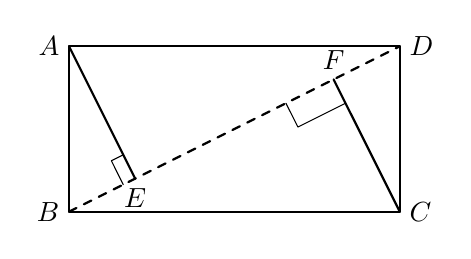
\begin{tikzpicture}[line cap=round,line join=round,scale=0.7]
\usetikzlibrary{calc}

% rectangle (wide)
\coordinate (B) at (0,0);
\coordinate (C) at (6,0);
\coordinate (D) at (6,3);
\coordinate (A) at (0,3);

\draw[thick] (A)--(B)--(C)--(D)--cycle;

% diagonal BD
\draw[dashed,thick] (B)--(D);

% feet E from A to BD, F from C to BD
\coordinate (E) at ($(B)!(A)!(D)$);
\coordinate (F) at ($(B)!(C)!(D)$);

\draw[thick] (A)--(E);
\draw[thick] (C)--(F);

% right angle marks at E and F w.r.t BD
\begin{scope}
  \coordinate (e1) at ($(E)!0.18!(B)$);
  \coordinate (e2) at ($(E)!0.18!(A)$);
  \coordinate (e3) at ($(e2)+(e1)-(E)$);
  \draw (e1) -- (e3) -- (e2);
\end{scope}
\begin{scope}
  \coordinate (f1) at ($(F)!0.18!(B)$);
  \coordinate (f2) at ($(F)!0.18!(C)$);
  \coordinate (f3) at ($(f2)+(f1)-(F)$);
  \draw (f1) -- (f3) -- (f2);
\end{scope}

% labels
\node[left] at (A) {$A$};
\node[left] at (B) {$B$};
\node[right] at (C) {$C$};
\node[right] at (D) {$D$};
\node[below] at (E) {$E$};
\node[above] at (F) {$F$};

\end{tikzpicture}

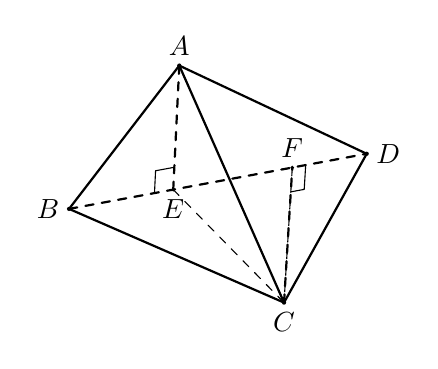
\begin{tikzpicture}[line cap=round,line join=round,scale=0.7]
\usetikzlibrary{calc}

% place points in a 2D perspective-like layout
\coordinate (B) at (0,0);
\coordinate (D) at (5.4,1.0);
\coordinate (C) at (3.9,-1.7);
\coordinate (A) at (2.0,2.6);

% E,F on BD (feet, schematic)
\coordinate (E) at ($(B)!0.35!(D)$);
\coordinate (F) at ($(B)!0.75!(D)$);

% faces edges (schematic)
\draw[thick] (B)--(A)--(D);
\draw[thick] (B)--(C)--(D);
\draw[thick] (A)--(C);

% fold line BD
\draw[dashed,thick] (B)--(D);

% perpendicular-ish segments (as in solution)
\draw[dashed,thick] (A)--(E);
\draw[dashed,thick] (C)--(F);

% auxiliary dashed inside
\draw[dashed] (E)--(C);
\draw[dashed] (F)--(C);

% right-angle marks at E,F (schematic)
\begin{scope}
  \coordinate (e1) at ($(E)!0.18!(B)$);
  \coordinate (e2) at ($(E)!0.18!(A)$);
  \coordinate (e3) at ($(e2)+(e1)-(E)$);
  \draw (e1) -- (e3) -- (e2);
\end{scope}
\begin{scope}
  \coordinate (f1) at ($(F)!0.18!(D)$);
  \coordinate (f2) at ($(F)!0.18!(C)$);
  \coordinate (f3) at ($(f2)+(f1)-(F)$);
  \draw (f1) -- (f3) -- (f2);
\end{scope}

% point marks + labels
\fill (A) circle (1.1pt) node[above] {$A$};
\fill (B) circle (1.1pt) node[left] {$B$};
\fill (C) circle (1.1pt) node[below] {$C$};
\fill (D) circle (1.1pt) node[right] {$D$};
\fill (E) circle (1.0pt) node[below] {$E$};
\fill (F) circle (1.0pt) node[above] {$F$};

\end{tikzpicture}

$B$，若存在某个位置，使得直线 $AB$ 与直线 $CD$ 垂直，则 $CD\perp$ 平面 $ABC$，平面 $ABC\perp$ 平面 $BCD$，取 $BC$ 中点 $M$，连接 $ME$，则 $ME\perp BD$，$\therefore \angle AEM$ 就是二面角 $A-BD-C$ 的平面角，此角显然存在，即当 $A$ 在底面上的射影位于 $BC$ 的中点时，直线 $AB$ 与直线 $CD$ 垂直，故 $B$ 正确；

$C$，若存在某个位置，使得直线 $AD$ 与直线 $BC$ 垂直，则 $BC\perp$ 平面 $ACD$，从而平面 $ACD\perp$ 平面 $BCD$，即 $A$ 在底面 $BCD$ 上的射影应位于线段 $CD$ 上，这是不可能的，排除 $C$；

$D$，由上所述，可排除 $D$．

故选 $B$．

先根据翻折前后的变量和不变量，计算几何体中的相关边长，再分别筛选四个选项，若 $A$ 成立，则需 $BD\perp EC$，这与已知矛盾；若 $B$ 成立，则 $A$ 在底面 $BCD$ 上的射影应位于线段 $BC$ 上，可证明位于 $BC$ 中点位置，故 $B$ 成立；若 $C$ 成立，则 $A$ 在底面 $BCD$ 上的射影应位于线段 $CD$ 上，这是不可能的；$D$ 显然错误．
\end{solutions}